\section{Untersuchung von Mikrowellen}

	\subsection{Methoden} \label{Methoden}
		
		Der Aufbau dieses Versuches variiert für die verschiedenen Teilversuche.
		Für alle jedoch werden elektromagnetische Wellen (im Mikrowellenbereich) von einem Sender ausgesendet und von einem Empfänger aufgefangen und die dortige Intensität als Spannung, das Strahlprofil, gemessen.
		
		\subsubsection*{Strahlendivergenz}
		\begin{figure}[ht]
			\centering
			\includegraphics[width=0.6\textwidth]{bilder/Mikrowelle_1.png}
			\caption{Aufbau zur Messung der Strahlendivergenz.\cite{WWU}}
			\label{fig:Aufbau1}	
		\end{figure}
	
		Zur Bestimmung der Strahlendivergenz wird wie in Abb. \ref{fig:Aufbau1} dargestellt, die Position des Empfängers über zwei Schienen verändert. 
		Jeweils eine horizontal und eine vertikal zu dem Sender liegende. 
		Damit lässt sich der virtuelle Quellfleck des Senders bestimmen.
		Die gemessenen Spannung sollen als Funktion des Ortes dargestellt werden. 
		
		\subsubsection*{Stehende Welle}
		\begin{figure}[ht]
			\centering
			\includegraphics[width=0.6\textwidth]{bilder/Mikrowelle_2.png}
			\caption{Aufbau zur Messung der Wellenlänge über eine stehende Welle.\cite{WWU}}
			\label{fig:Aufbau2}	
		\end{figure}
		Für die Erzeugung einer stehenden Welle wird eine Metallplatte gegenüber dem Sender platziert. 
		Dies ist in Abb. \ref{fig:Aufbau2} dargestellt.
		Der Empfänger liegt hierbei zwischen Sender und Metallplatte. 
		Bei stehenden Wellen ist an den Knotenpunkten für jede Zeit der gleiche Wert zu messen.
		Deswegen wird der Abstand zwischen Sender und Metallplatte so angepasst, dass sich solche Knotenpunkte mit dem Empfänger finden lassen.
		An der Metallplatte muss dafür ein Knoten liegen und der Abstand zweier Knoten entspricht einer halben Wellenlänge.
		Diese lässt sich also über das Messen zweier Knotenpunkte bestimmen.
		
		\subsubsection*{Brechungsindexbestimmung}
		\begin{figure}[ht]
			\centering
			\includegraphics[width=0.6\textwidth]{bilder/Mikrowelle_3.png}
			\caption{Aufbau zur Bestimmung des Brechungsindexes von PVC.\cite{WWU}}
			\label{fig:Aufbau3}	
		\end{figure}
		Danach soll ein PVC-Halbzylinder untersucht werden. 
		Dieser befindet sich wie in Abb. \ref{fig:Aufbau3} zu sehen fixiert über einer mit einer Schiene verbundenen drehbaren Platte auf der Winkel eingezeichnet sind.
		So lässt sich nach dem Snellius'schen Brechungsgesetz
		\begin{equation} \label{eq:snell}
			n_1 \sin{\phi_1} = n_2 \sin{\phi_2}
		\end{equation}
		der Brechungsindex $n_\text{PVC}$ des Halbzylinders bestimmen. 
		Die benötigten Winkel dafür lassen sich der drehbaren Platte entnehmen und der Brechungsindex von Luft $n_\text{Luft}$ entspricht in etwa 1.
		
		\subsubsection*{Frustrierte Totalreflexion}
		\begin{figure}[ht]
			\centering
			\includegraphics[width=0.6\textwidth]{bilder/Mikrowelle_4.png}
			\caption{Aufbau zur Messung der Intensität bei frustrierte Totalreflexion.\cite{WWU}}
			\label{fig:Aufbau4}	
		\end{figure}
		Für den Winkel $\phi_\text{PVC}$, bei dem $\phi_\text{Luft}$ bei \SI{90}{\degree} liegt, tritt das Phänomen der Totalreflexion auf, was bedeutet, dass die elektromagnetische Welle keinen transmittierten Teil mehr besitzt, sondern vollständig an der Grenzfläche reflektiert wird. 
		Da die elektromagnetische Welle jedoch eine gewisse "Breite" besitzt, breitet diese sich nahe der Grenzfläche, wenn auch exponentiell abfallend in dem angrenzenden Medium aus.
		Diesen Teil nennt man evaneszente Welle.
		Bringt man ein weiteres Medium mit größerem Brechungsindex näher, so wird diese evaneszente Welle in diesem Medium "zurückgebrochen" und breitet sich darin weiter aus.
		Diese "frustrierte" Totalreflexion soll für diesen Versuch mit einem zweiten PVC-Halbzylinder veranschaulicht und gemessen werden. 
		Dazu Abb. \ref{fig:Aufbau4}.
		Die gemessene Intensität an dem Empfänger soll zudem in Abhängigkeit des Abstands der Zylinder aufgetragen werden.		
		
		\subsubsection*{Bragg'sche Reflexion}
		\begin{figure}[ht]
			\centering
			\includegraphics[width=0.6\textwidth]{bilder/Mikrowelle_5.png}
			\caption{Aufbau zur Bestimmung des Gitterabstandes der Metallkugeln in dem Schaumstoffquader.\cite{WWU}}
			\label{fig:Aufbau5}	
		\end{figure}
		Zuletzt soll ein Metallkugelgitter in einem Schaumstoffquader untersucht werden (vgl. Abb. \ref{fig:Aufbau5}). 
		Dieser liegt auf der drehbaren Platte und zwar so, dass bei dem Drehen der Schiene der Quader so mitgedreht wird, dass für Sender und Empfänger immer Einfallswinkel $\alpha$ = Ausfallswinkel gilt.
		Über die Bragg'sche Reflexion
		\begin{equation} \label{eq:bragg}
			2d\sin{\alpha} = n\lambda
		\end{equation}
		lässt sich der Abstand zwischen den Gitterebenen $d$ bestimmen.
		Zur Veranschaulichung dient Abb. \ref{fig:bragg}.
		\begin{figure}[ht]
			\centering
			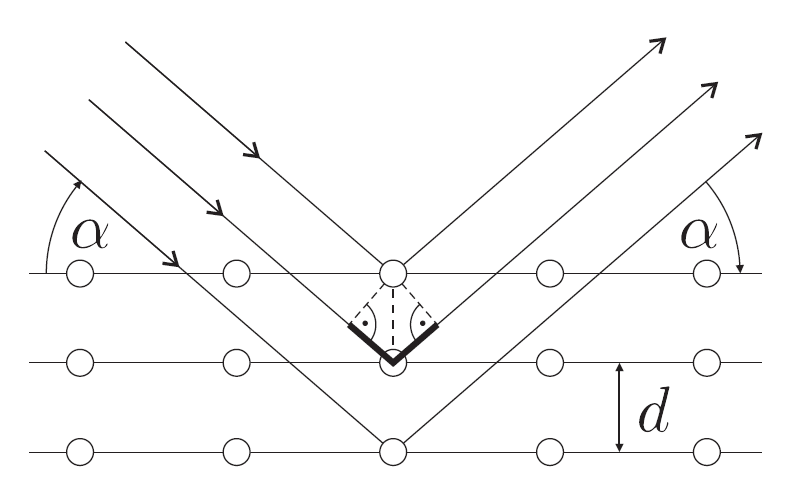
\includegraphics[width=0.6\textwidth]{bilder/Bragg.png}
			\caption{Darstellung des Metallkugelgitters und den für die Bragg'sche Reflexion relevanten Größen.\cite{WWU}}
			\label{fig:bragg}	
		\end{figure}
		Der sogenannte Glanzwinkel $\alpha_\text{g}$ wird durch Drehung der Platte und Intensitätsmessung an dem Empfänger festgelegt und die zuvor bestimmte Wellenlänge zur Bestimmung des Gitterabstandes $d$ verwendet. 
		
	\subsection{Durchführung}
	
		Alle in Abschnitt \ref{Methoden} dargestellten Teilversuche wurden durchgeführt.
		Bei den Messungen traten keine Komplikationen auf.
		Einzelne Messwerte sind dem Laborbuch zu entnehmen.
		Für die Strahlendivergenz wurde die in Abb. \ref{fig:divergenz} dargestellte Intensitätsverteilung aufgenommen. 
		\begin{figure}[ht]
			\centering
			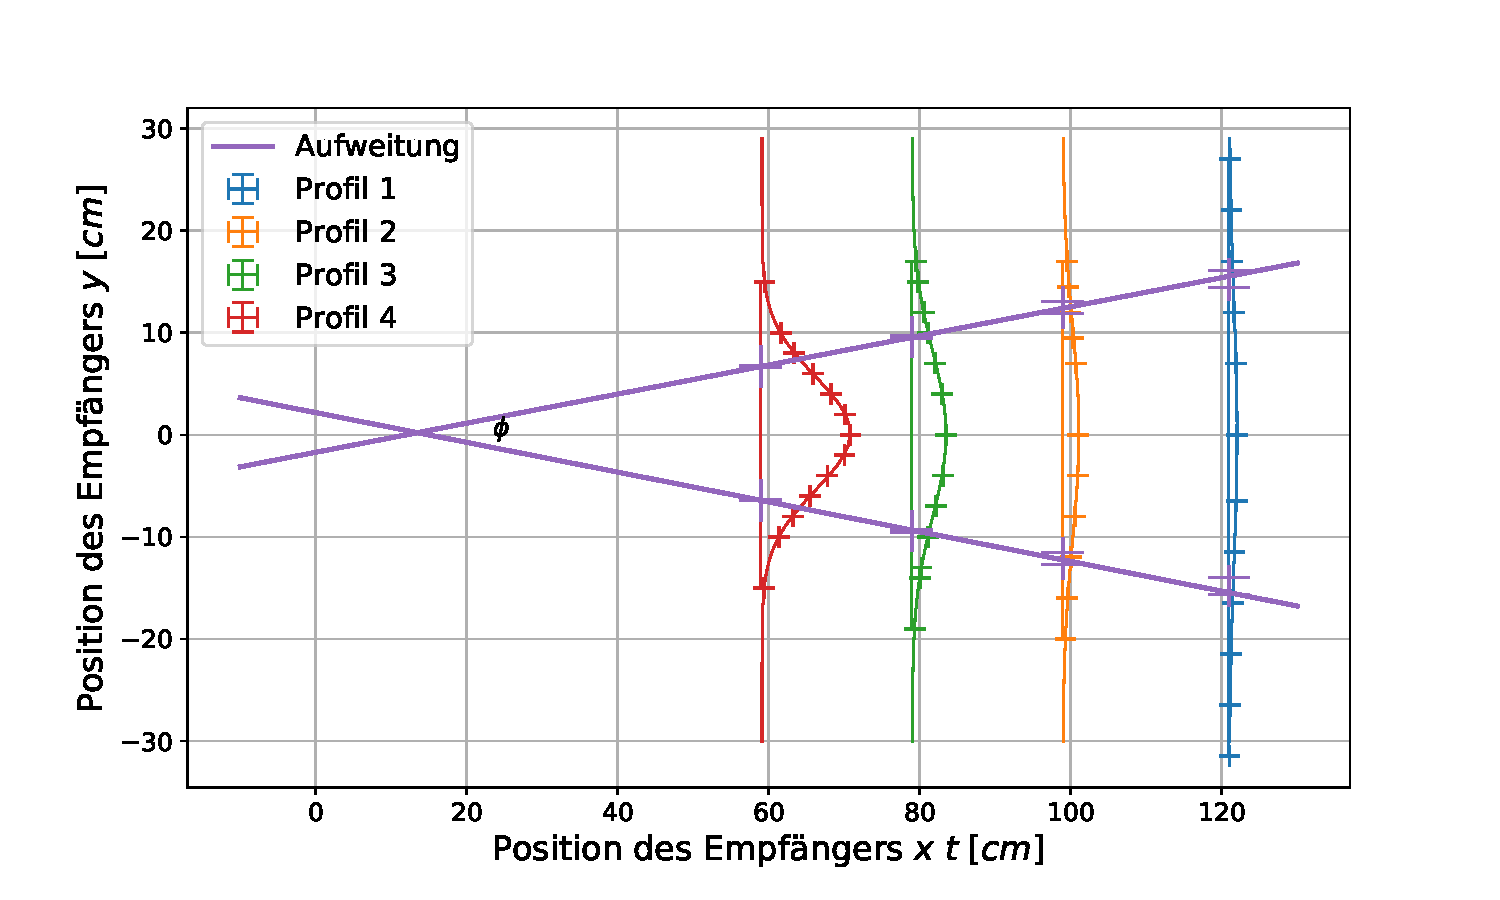
\includegraphics[width=\textwidth]{data/profil.pdf}
			\caption{Gemessene Strahlenprofile für die verschiedenen Abstände des Empfängers von dem Sender. Mit Gauß-Kurven gefittet (Fit-Details im Anhang).}
			\label{fig:divergenz}	
		\end{figure}
	
		\begin{table}[ht]
			\centering
			\begin{tabular}{r|SSSS}
				\hline
				& $x_0$ & $A$ & $d$ & $y_0$ \\
				\hline
				{Profil 1} & \SI{0.21+-0.30}{\centi\meter} & \SI{1.04+-0.04}{\volt} & \SI{12.8+-0.7}{\centi\meter} & \SI{0.05+-0.04}{\centi\meter}\\
				{Profil 2} & \SI{0.18+-0.13}{\centi\meter} & \SI{2.12+-0.10}{\volt} & \SI{10.4+-0.5}{\centi\meter} & \SI{0.02+-0.10}{\centi\meter}\\
				{Profil 3} & \SI{0.07+-0.05}{\centi\meter} & \SI{4.45+-0.06}{\volt} & \SI{8.07+-0.13}{\centi\meter} & \SI{0.08+-0.06}{\centi\meter}\\
				{Profil 4} & \SI{0.143+-0.027}{\centi\meter} & \SI{11.68+-0.08}{\volt} & \SI{5.56+-0.05}{\centi\meter} & \SI{0.16+-0.07}{\centi\meter}\\
				\hline
			\end{tabular}
			\caption{Fit-Parameter der Strahlprofile mit $y = A \exp\left\lbrace \frac{(x-x_0)^2}{2 d^2} \right\rbrace + y_0$.}
			\label{tab:strahlendivFit}
		\end{table}

		Zur Bestimmung der Wellenlänge, wurden bei dem Teilversuch mit der stehenden Welle vier Minima verzeichnet.
		Der mittlere Abstand dieser betrug \SI{1,567+-0,009}{\centi\meter}.
		Um den Brechungsindex des PVC-Halbzylinders zu bestimmen, wurden fünf verschiedene Einfallswinkel, in \SI{10+-1}{\degree} Abständen, und die zugehörigen Winkel des transmittierten Strahl aufgenommen.
		Nachdem einstellen des Winkels, für den die Totalreflexion eintrat, wurde ein zweiter PVC-Zylinder herangezogen und die Intensität hinter diesem für acht Abstände in \SI{0,5+-0,21}{\centi\meter} Schritten gemessen.
		Diese Intensität ist in Abb. \ref{fig:totalreflexion} dargestellt.
		Es lässt sich ein exponentieller Abfall erkennen.
		\begin{figure}[ht]
			\centering
			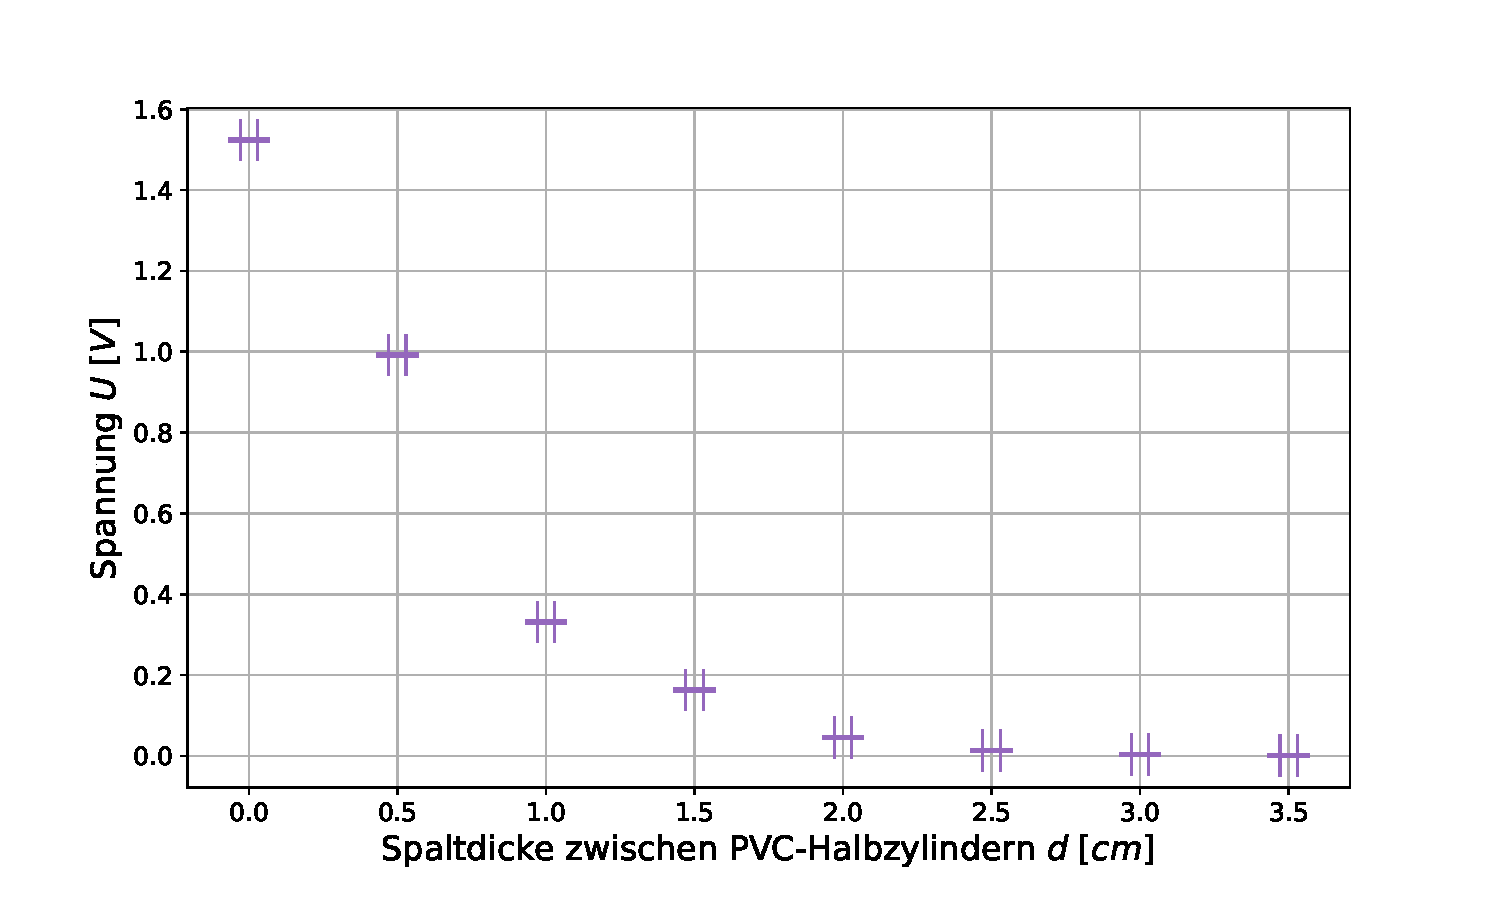
\includegraphics[width=\textwidth]{data/totalreflektion.pdf}
			\caption{Intensität an dem Empfänger in Abhängigkeit des Abstandes der beiden PVC-Halbzylinder.}
			\label{fig:totalreflexion}	
		\end{figure}
		Um den Glanzwinkel $\alpha_\text{g}$ bei dem Teilversuch mit dem Metallkugelgitter in dem Schaumstoffquader genau bestimmen zu können wurden die Intensitäten bei Winkeln $\alpha$ auf der drehbaren Platte von \SIrange{5+-1}{80+-1}{\degree} aufgenommen.
		Bei Winkeln von \SI{38+-1}{\degree} und \SI{75+-1}{\degree} waren Maxima in der Intensität zu erkennen (vgl. Abb.\ref{fig:braggwinkel}).
		\begin{figure}[ht]
			\centering
			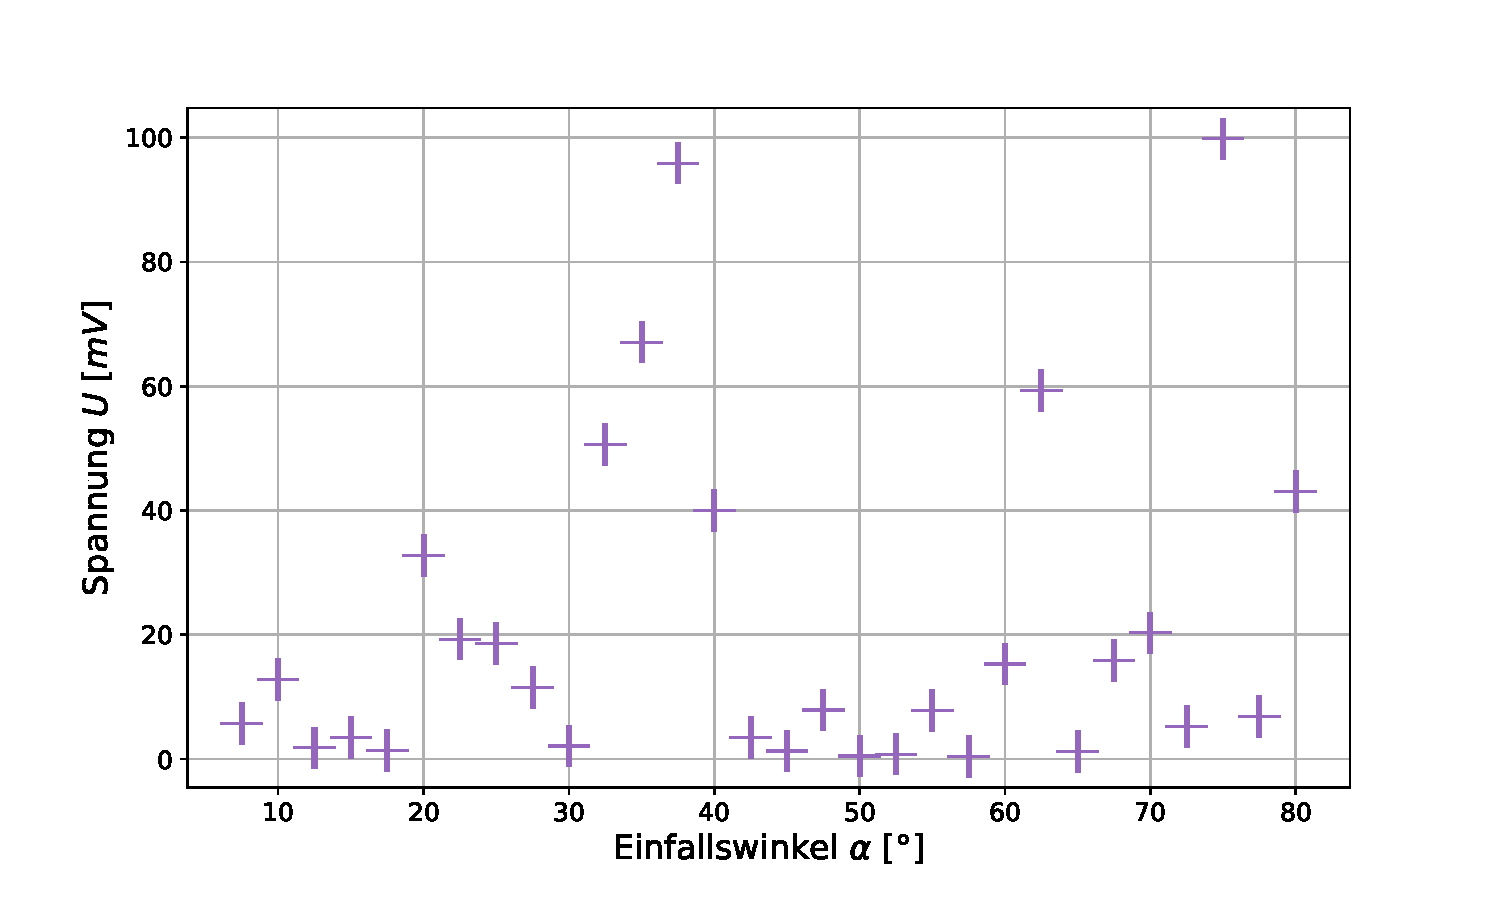
\includegraphics[width=\textwidth]{data/schaumstoff.pdf}
			\caption{Intensitätsspektrum bei der Gitterreflexion in Abhängigkeit des Winkels $\alpha$.}
			\label{fig:braggwinkel}	
		\end{figure}
		Zum Vergleich wurde zusätzlich der Abstand zweier Metallkugeln gemessen, dieser belief sich auf \SI{3,8+-0,02}{\centi\meter} 
		
	\subsection{Datenanalyse}
		
		Über die verwendeten Gauß-Kurven Fits in Abb. \ref{fig:divergenz} ließ sich der Quellpunkt der elektromagnetischen Welle auf \SI{13.5+-1.1}{\centi\meter} vor der Befestigung des Senders ermitteln.
		Zudem ließ sich die in der Abbildung dargestellte Aufweitung $\phi$ auf einen Winkel von \SI{16.41+-0.28}{\degree} bestimmen.
		Es wurden Gauß-Kurven für den Fit gewählt, da alle Messwerte für die vier Abstände in $x$-Richtung sich auf diesen auffinden ließen. 
		Für einen anderen Fit würden die Unsicherheiten für den Quellpunkt zu groß werden, als dass sich eine Aussage über seine Position tätigen ließe. % behaupte ich mal, besser iwas erwähnen als nichts
		Da die Wellenlänge sich aus dem doppelten Abstand zweier nebeneinander liegenden Minima bestimmt, ergab sich, aus dem mittleren Abstand der Minima, für die Mikrowelle eine Wellenlänge von $\lambda = \SI{3.133+-0.019}{\centi\meter}$. 
		Unter der Annahme, dass der Brechungsindex von Luft $n_\text{Luft}\approx 1$ ist, ergibt das Mittel der fünf über \ref{eq:snell} berechneten Brechungsindizes, dass der PVC-Halbyzylinder einen Brechungsindex von $n_\text{PVC} = \SI{1.66+-0.17}{}$ besitzt.
		Aus den Messwerten für die frustrierte Totalreflexion (vgl. Abb. \ref{fig:totalreflexion}), lässt sich ein exponentieller Abfall mit steigendem Abstand der Halbzylinder erkennen.
		Dies deckt sich mit dem exponentiellen Abfall in dem angrenzendem Medium bei der einfachen Totalreflexion.
		Einsetzen der beiden ermittelten Glanzwinkel $\alpha_{\text{g},1/2}$ in Gl. \ref{eq:bragg} liefert Abstände der Netzebene von $d_1 = \SI{2.574+-0.017}{\centi\meter}$ und $d_2 = \SI{3.244+-0.020}{\centi\meter}$, welche jedoch gleich sein sollten.
		
	\subsection{Diskussion}
	
		Nun stellt sich die Frage, ob die ermittelten Werte die Hypothese stützen, dass sie alle mit der Literatur übereinstimmen.
		Da sich für den Brechungsindex von PVC ein Literaturwert finden ließ, bietet es sich an diesen zunächst mit der Ermittlung zu vergleichen.
		Dieser Literaturwert\cite{GF} beläuft sich auf $n_\text{PVC} = \SI{1,54}{}$, der ermittelte hingegen auf $n_\text{PVC} = \SI{1.66+-0.17}{}$. 
		Der Literaturwert liegt also innerhalb der aufgrund der Mittelung recht großen Unsicherheit des berechneten Wertes.
		So lässt sich eine Übereinstimmung mit der Literatur an dieser Stelle definitiv nicht ausschließen.
		Bei der Betrachtung der Strahlendivergenz fällt logischerweise zunächst auf, dass die Intensität je weiter der Empfänger von dem Sender entfernt ist auch schwächer ist.
		Diese Intensität scheint zwischen quadratisch und exponentiell auseinander zu laufen, dies diente zum Anlass verschiedene Fits über die Messpunkte zu legen, welche ein solches Verhalten aufweisen (Lorentz, Gauß).
		Zudem sind der virtuelle Quellfleck und die Aufweitung, die sich durch den passenderen Gauß-Fit ergeben haben insofern sinnvoll, dass diese sich mit dem "Trichter", welcher auf dem Sender liegt (vgl. Abb. in \ref{Methoden}), decken..
		Da Mikrowellen in dem Wellenlängenbereich zwischen \SI{1}{\milli\meter} und \SI{30}{\centi\meter} liegen, lässt sich eindeutig sagen, dass die hier berechnete Wellenlänge von $\lambda = \SI{3.133+-0.019}{\centi\meter}$ in diesem Bereich liegt und demnach auch tatsächlich "Mikrowellen" untersucht wurden. 
		Die Betrachtung der frustrierten Totalreflexion lieferte ebenfalls das gewünschte Ergebnis eines exponentiellen Abfalls in Abhängigkeit des Abstandes der beiden PVC-Halbzylinder.
		Bei der Bragg'schen Reflexion an dem Metallkugelgitter hingegen lässt sich keine  genaue Aussage treffen, hier wurden zwei verschiedene Gitterabstände ermittelt $d_1 = \SI{2.574+-0.017}{\centi\meter}$ und $d_2 = \SI{3.244+-0.020}{\centi\meter}$, die weit außerhalb ihrer Unsicherheiten liegen.
		Fehlerquellen könnten einer falschen Einstellung der Drehplatte und der Schienen entspringen, sind jedoch eigentlich auszuschließen, da Einfallswinkel gleich Ausfallswinkel mit den verwendeten Einstellungen garantiert war.
		Ein schiefes Aufsetzten des Schaumstoffquaders ist aufgrund der Aufsatzfläche auch eher unwahrscheinlich.
		Von dem gemessenen Wert des Gitterabstands von \SI{3,8+-0,02}{\centi\meter} liegt $d_2$ deutlich näher als $d_1$, jedoch immer noch weit von dem gemessenen Wert (ca. 16\% Abweichung).
		Wie bereits erwähnt, lässt sich hierbei keine genaue Aussage treffen. 
		